\documentclass[8pt]{article}
\usepackage[utf8]{inputenc}
% http://texdoc.net/texmf-dist/doc/latex/geometry/geometry.pdf
% https://mike42.me/blog/2016-01-how-to-arrange-pages-for-printing-and-cutting-in-latex

%Font
\usepackage[]{roboto} 

\renewcommand*\familydefault{\sfdefault} 	
\usepackage[T1]{fontenc}
\usepackage{hyperref}

\usepackage{array}

\newcolumntype{x}[1]{%
>{\raggedleft\hspace{0pt}}p{#1}}%
% more font size definitions
\usepackage{moresize}	

\usepackage[paperwidth=85mm, paperheight=55mm, margin=3mm, showcrop=true]{geometry}
\usepackage{tikz}
\usetikzlibrary{shapes, backgrounds}

\usepackage{graphicx}
\usepackage{wrapfig}
\usepackage{ragged2e}

% use to vertically center content
% credits to: http://tex.stackexchange.com/questions/7219/how-to-vertically-center-two-images-next-to-each-other
\newcommand{\vcenteredinclude}[1]{\begingroup
\setbox0=\hbox{\includegraphics{#1}}%
\parbox{\wd0}{\box0}\endgroup}

% use to vertically center content
% credits to: http://tex.stackexchange.com/questions/7219/how-to-vertically-center-two-images-next-to-each-other
\newcommand*{\vcenteredhbox}[1]{\begingroup
\setbox0=\hbox{#1}\parbox{\wd0}{\box0}\endgroup}

% draw a circle with facts
% param 1: fact text
% param 2: scale default=1 (scales only chart, not label text)
% param 3: big border color
% param 4: second border color
% param 5: label bg color
\newcommand{\factbubble}[5]{
	\begin{tikzpicture}
	\pgfmathparse{#2*2}
	\let\pbxwidth\pgfmathresult
		\filldraw[fill=#3,draw=none] (0,0) circle (#2 * 1.5);
		\filldraw[fill=#5,draw=#4, line width=3.5pt] (0,0) circle (#2 * 1.2);
		\node at (0,0) {
			\parbox{\pbxwidth cm}{
				\begin{center}	
					#1
				\end{center}
			}
		};
	\end{tikzpicture}
}

\usepackage{color}
\definecolor{maincol}{HTML}{1B6D99}
\definecolor{secondcol}{HTML}{FCA311}
\definecolor{thirdcol}{HTML}{5CC8FF}
\definecolor{fourthcol}{HTML}{0B1F49}
\definecolor{fifthcol}{HTML}{eac381}
\definecolor{sixthcol}{RGB}{0,0,0}
\definecolor{textcol}{HTML}{000000}

%background color
\definecolor{bgcol}{HTML}{FFFFFF}%227,217,207}

%textcolor
%\definecolor{textcol}{HTML}{4B4E6D}

%sectioncolor
\definecolor{sectcol}{HTML}{FFFFFF}

%set a background col for whole page
\pagecolor{bgcol}

\newcommand{\icons}{Font-Awesome-SVG-PNG/}	%path to your icon lib
\newcommand{\icon}[2]{\colorbox{secondcol}{\includegraphics[height=#2]{\icons#1}}}	%icon shortcut
\newcommand{\icontext}[4]{ 						%icon with text shortcut
	\vcenteredhbox{\icon{#1}{#2}}\hspace{#4} \vcenteredhbox{\textcolor{textcol}{#3}}
	%\vcenteredhbox{\textcolor{textcol}{#3}} \hspace{5pt} \vcenteredhbox{\icon{#1}{#2}} \hspace{20pt}
}

\usepackage[cam,width=91truemm, height=61truemm,pdftex,center]{crop}
\begin{document}
\small
        \begin{flushleft}
            \colorbox{maincol}{\large{\textcolor{white}{\textbf{\uppercase{Arianne Meijer}}} }}\\
            \small{\textcolor{fourthcol}{\textsc{Pocket Resume}}}\\
            \end{flushleft}
            \vspace{-10pt}
            \parbox{0.6\textwidth}{
            \begin{flushleft}
            \small
			\icontext{at2}{10pt}{\href{mailto:ariannemeijer@gmail.com}{ariannemeijer@gmail.com} }{5pt}\\[-2pt]
			\icontext{mobile-phone2}{10pt}{+358 45 31 296 31}{5pt}\\[-2pt]
			\icontext{map-marker2}{10pt}{Espoo, Finland}{5pt}\\[-2pt]
			\icontext{linkedin-box2}{10pt}{\href{https://linkedin.com/in/aerylia}{linkedin.com/in/aerylia}}{5pt}
			\end{flushleft}
			}
			\parbox{0.4\textwidth}{
			\begin{center}
			\vspace{-20pt}
			\colorbox{fourthcol}{\includegraphics[height=10pt]{\icons download}\hspace{5pt} \textcolor{white}{Full resume}}\\
			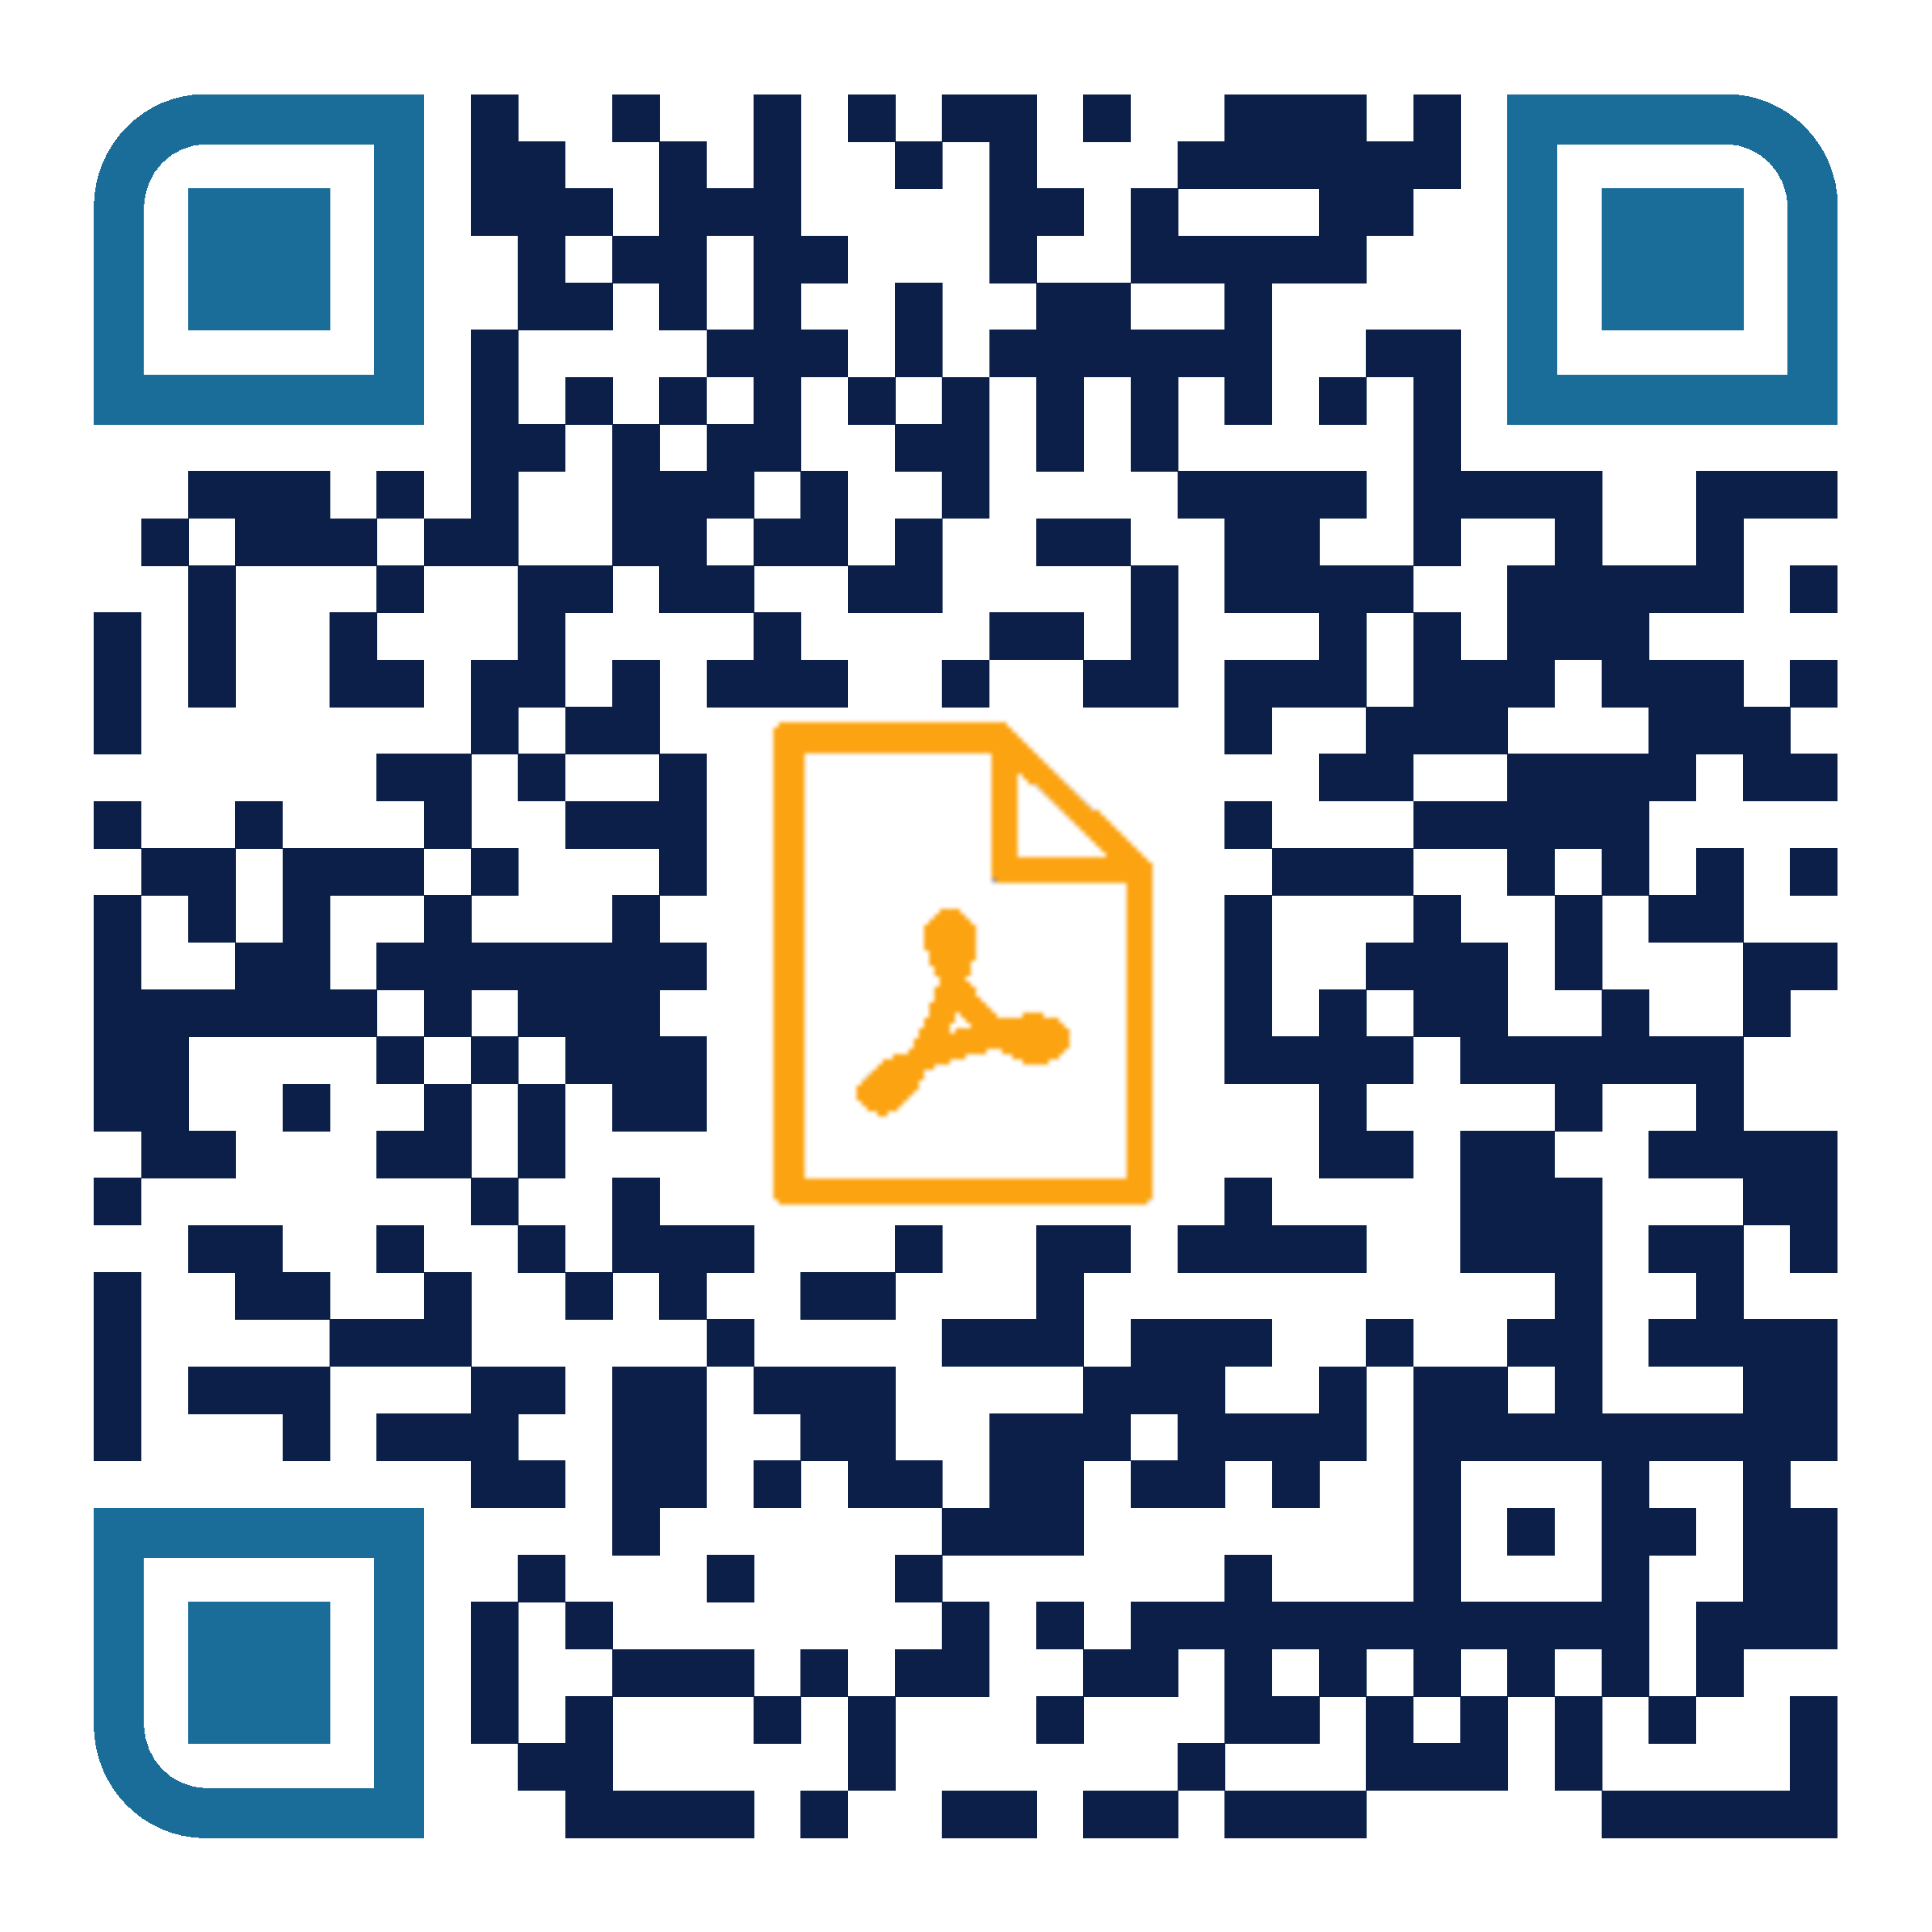
\includegraphics[height=75pt]{qr-code2.pdf}
			\end{center}
			}
			\begin{center}
			\vspace{-10pt}
			%\colorbox{thirdcol}{\ssmall{\textcolor{white}{\textsc{Student at Radboud University Nijmegen.}} }} \\[-2pt]
			%\colorbox{thirdcol}{\hspace{13pt}\small{\textcolor{white}{Graduate Student \textbf{Msc. Computer Science \& A.I.}}\hspace{13pt}}}
			\colorbox{thirdcol}{\hspace{3pt}\small{\textcolor{white}{\textbf{Computer Science PhD student, NISQ Software}}\hspace{2pt}}}
			\end{center}
\newpage
        \begin{center}
            \colorbox{maincol}{\large{\textcolor{white}{\textbf{T}}}\small{\textcolor{white}{oo}} \large{\textcolor{white}{\textbf{L}}}\small{\textcolor{white}{ong}} \large{\textcolor{white}{\textbf{; D}}}\small{\textcolor{white}{idn't}} \large{\textcolor{white}{\textbf{R}}}\small{\textcolor{white}{emember}}}\\
        \end{center}
        \ssmall
        \begin{flushleft}
            %\icontext{square-solid}{5pt}{\textcolor{fourthcol}{\textbf{Looking for an AI Master thesis project February - July 2019}}}{3pt}\\[2pt]
            \icontext{square-solid}{5pt}{\textcolor{fourthcol}{\textbf{Interested in fun and challenging problems to solve in new creative ways}}}{3pt}\\[2pt]
            \icontext{square-solid}{5pt}{\textcolor{fourthcol}{\textbf{Languages:}} Dutch (native), English (professional), German (intermediate)}{3pt}\\[2pt]
            \icontext{square-solid}{5pt}{\textcolor{fourthcol}{\textbf{Languages:}} Python (native), Java (advanced), C (basic), Haskell/Clean (basic)}{3pt}\\[2pt]
            \icontext{square-solid}{5pt}{\textcolor{fourthcol}{\textbf{Worked at:}} Atos, RadboudUMC, Anchormen, SIMON, Machine2Learn}{3pt}\\[2pt]
            \icontext{square-solid}{5pt}{\textcolor{fourthcol}{\textbf{Interests:}} Quantum Computing, Machine Learning, Neural Networks, NLP}{3pt}\\[2pt]
            \icontext{square-solid}{5pt}{\textcolor{fourthcol}{\textbf{Hobbies:}} Knitting, Netflix, Logic puzzles, Sewing, Hackathons, Anime}{3pt}\\[2pt]
            \icontext{square-solid}{5pt}{\textcolor{fourthcol}{\textbf{Obtained degrees:}} Msc. Computer Science \& Artificial Intelligence (cum laude)}{3pt}\\[2pt]
            \icontext{square-solid}{5pt}{\textcolor{fourthcol}{\textbf{Expected graduation:}} December 2024, CS PhD student}{3pt}\\[2pt]
            \icontext{square-solid}{5pt}{\textcolor{fourthcol}{\textbf{Resume in QR code will stay up-to-date}} }{3pt}\\[2pt]
        \end{flushleft}
        \begin{flushright}
        \vspace{-25pt}
        ORCID ID:\\
			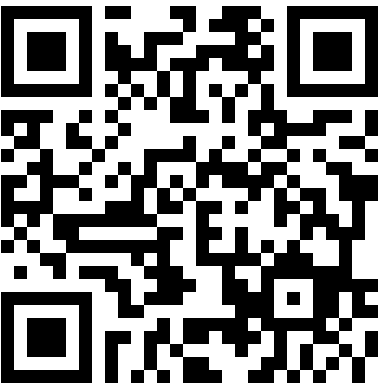
\includegraphics[height=50pt]{ORCID_QR_code.png}
        \end{flushright}
        \vspace{-25pt}
			\colorbox{thirdcol}{\hspace{3pt}\small{\textcolor{white}{\textbf{University of Helsinki}}\hspace{2pt}}}
\end{document}
